\documentclass[11pt,twoside]{article}

\usepackage{blindtext}
\usepackage[T1]{fontenc}
\usepackage{microtype}
\usepackage[english]{babel}
\usepackage[hmarginratio=1:1,top=32mm,columnsep=20pt,left=2cm]{geometry}
\usepackage[hang, small,labelfont=bf,up,textfont=it,up]{caption}
\usepackage{booktabs}
\usepackage{lettrine}
\usepackage{enumitem}
\setlist[itemize]{noitemsep}
\usepackage{graphicx}

\usepackage{abstract}
\renewcommand{\abstractnamefont}{\normalfont\bfseries}
\renewcommand{\abstracttextfont}{\normalfont\small}

\usepackage{titlesec}
\titleformat{\section}[block]{\large\scshape\centering}{\thesection.}{1em}{}
\titleformat{\subsection}[block]{\large}{\thesubsection.}{1em}{}
\usepackage{titling}
\usepackage{hyperref}

%----------------------------------------------------------------------------------------
%   TITLE SECTION
%----------------------------------------------------------------------------------------

\setlength{\droptitle}{-4\baselineskip} % Move the title up

\pretitle{\begin{center}\Huge\bfseries} % Article title formatting
\posttitle{\end{center}} % Article title closing formatting
\title{Machine Learning} % Article title
\author{%
\textsc{Gianmarco Ricciarelli} \\[1ex] % Your name
\normalsize \href{mailto:john@smith.com}{gianmarcoricciarelli@gmail.com} % Your email address
\and % Uncomment if 2 authors are required, duplicate these 4 lines if more
\textsc{Stefano Carpita} \\[1ex] % Second author's name
\normalsize \href{mailto:jane@smith.com}{carpitastefano@gmail.com} % Second author's email address
}
\date{
    ML - Academic Year: 2018/2019 \\
    {\vspace{0.25cm}}
    \today \\
    {\vspace{0.25cm}}
    Type of project: \textbf{A} \\
    {\vspace{0.25cm}}
    \href{https://github.com/germz01/machinel-learning}{Github Page}
}
\renewcommand{\maketitlehookd}{%
\begin{abstract}
\noindent With this report we describe our type \textbf{A} project for the Machine Learning course. We experiment
two datasets, namely MONK's and CUP, by building from scratch a neural network's implementation, which we've
validated by searching for the best hyper-parameters' combination via well-known validation techniques. Finally,
for each one of the datasets, we collected the data describing the results.
\end{abstract}
}

%----------------------------------------------------------------------------------------

\begin{document}

% Print the title
\maketitle

%----------------------------------------------------------------------------------------
%   ARTICLE CONTENTS
%----------------------------------------------------------------------------------------

\section{Introduction} % (fold)
\label{sec:introduction}
    By chosing the type \textbf{A} project, we followed the goal of optimizing a built from scratch neural
    network model by searching for the best hyper-parameters' combination in order to obtain the best
    performances on the MONK's and CUP datasets. The model we've built implements the
    standard \textit{backpropagation algorithm} with \textit{gradient descent}, as described in
    \cite{deep_learning}. As optimization tool, we've searched the so-called hyper-parameters space by using
    well-known validation algorithms like \textit{k-fold cross validation} and \textit{grid search},
    described in \cite{deep_learning} and \cite{random_search}. More technical details about the
    implementation can be found in section \ref{sec:methods}.
% section introduction (end)

%------------------------------------------------

\section{Methods} % (fold)
\label{sec:methods}
    Our code base is written using the \textit{Python} programming language, which was enhanced with
    numerical libraries like \textit{NumPy} and \textit{Pandas} to ease the computational cost involved in
    implementating popular machine learning algorithms. Also the standard library function provided by the
    language were utilized. Following the philosophy of type \textbf{A} projects, we haven't used
    out-of-the-box implementations for the algorithms composing our framework. We now give a brief overview of
    the code's structure, discuss some implementation choices and present our neural network's initialization
    and training algorithms. Visit the project's
    \href{https://github.com/germz01/machinel-learning}{\underline{\textit{Github Page}}} if you want to check
    our project's code base.

    \subsection{Code overview} % (fold)
    \label{sub:code_overview}
        We can view our code base essentialy divided in two branches: the \textit{neural network} branch and
        the \textit{model selection and assessment} branch. The first one is composed by the code for
        implementing the neural network model, and all the code related
        to the building and training of such a model, e.g. the activation functions, the losses, the
        regularization metrics and so on, that is divided in several scripts in order to ease the
        implementation. The code base's second branch consist in the model selection and assessment related
        code, which is composed by several classes, each one implementing an algorithm like \texttt{GridSearch}
        and \texttt{KFold\_Cross\_validation} which are utilized for the model's validation, selection and
        assessment, and the scripts that build up the testing routines for the MONK's and CUP datasets.
        The second branch also is splitted in several scripts.
    % subsection code_overview (end)

    \subsection{Implementation choices} % (fold)
    \label{sub:implementation_choices}
        Since we wanted to be able to take different paths during the building phase of our model, we enriched
        the first code base's branch by writing diffent activation functions, losses and regularization metrics.
        In the \texttt{activation} script we writed the code for the \texttt{sigmoid}, \texttt{relu},
        \texttt{tanh} and \texttt{identity} activation functions. The \texttt{regularizers} script contains the
        code for implementing both the $L^1$ and $L^2$ regularization metrics, as described in
        \cite{deep_learning}, and the \texttt{losses} script contains the code for implementing popular loss
        function like, for example, the \texttt{mean\_squared\_error} and the \texttt{mean\_euclidean\_error}.
        All this metrics are applied in the \texttt{nn} script, which contains the code for implementing the
        neural network model, and hence the backpropagation algorithm and the training algorithm, described in
        section \ref{sub:the_training_algorithm}. The \texttt{NeuralNetwork} class, which is contained in this
        script, represents a neural network using the standard \textit{backpropagation algorithm} with
        \textit{gradient descent}, \textit{standard momentum} and \textit{regularization}, and follows the
        \textit{minibatch} approach, as described in \cite{deep_learning}. The \texttt{NeuralNetwork} class
        contains also various early stopping metrics, like the $GL_{\alpha}$ and the $PQ_{\alpha}$ which we
        implemented following \cite{early_stopping}. More details about what particular combination of
        metrics was used during the experimental phase can be found in section \ref{sec:experiments}.

        \subsection{Network's initialization and training} % (fold)
        \label{sub:the_training_algorithm}
        Our neural network can be initialized for pursuing either a \textit{classification} task or a
        \textit{regression} one. The initialization phase for the two tasks is the same.
        During the initialization phase, we pass to the network the design matrix \texttt{X} and target column
        vector \texttt{y}. Other than that we pass the number of neurons per hidden layer
        \texttt{hidden\_sizes}, the maximum number of epochs \texttt{epochs}, the minibatch's size
        \texttt{batch\_size}, the activation function for each layer \texttt{activation} and the
        hyper-parameters for the learning rate, \texttt{$\eta$}, the momentum, \texttt{$\alpha$} and the
        regularization, \texttt{$\lambda$}. In order to initialize the network's weights matrices we've
        followed the \textit{normalized initialization} technique, as described in \cite{deep_learning} and
        \cite{initialization}. During the training phase we essentialy apply the \textit{forward propagation}
        and the \textit{backpropagation} phases of the standard \textit{backpropagation} algorithm over a
        minibatch of examples taken from the training set. During each epoch of training we also keep track of
        the errors between the predicted values and target ones, in order to be able to plot the
        \textit{learning curves} for the training session. At the end of each epoch the neural network's
        weights are updated following the standard backpropagation/momentum/regularization convention.
        % subsection the_training_algorithm (end)
    % subsection implementation_choices (end)
% section methods (end)

%------------------------------------------------

\section{Experiments} % (fold)
\label{sec:experiments}

\begin{figure}[htbp]
  \centering
  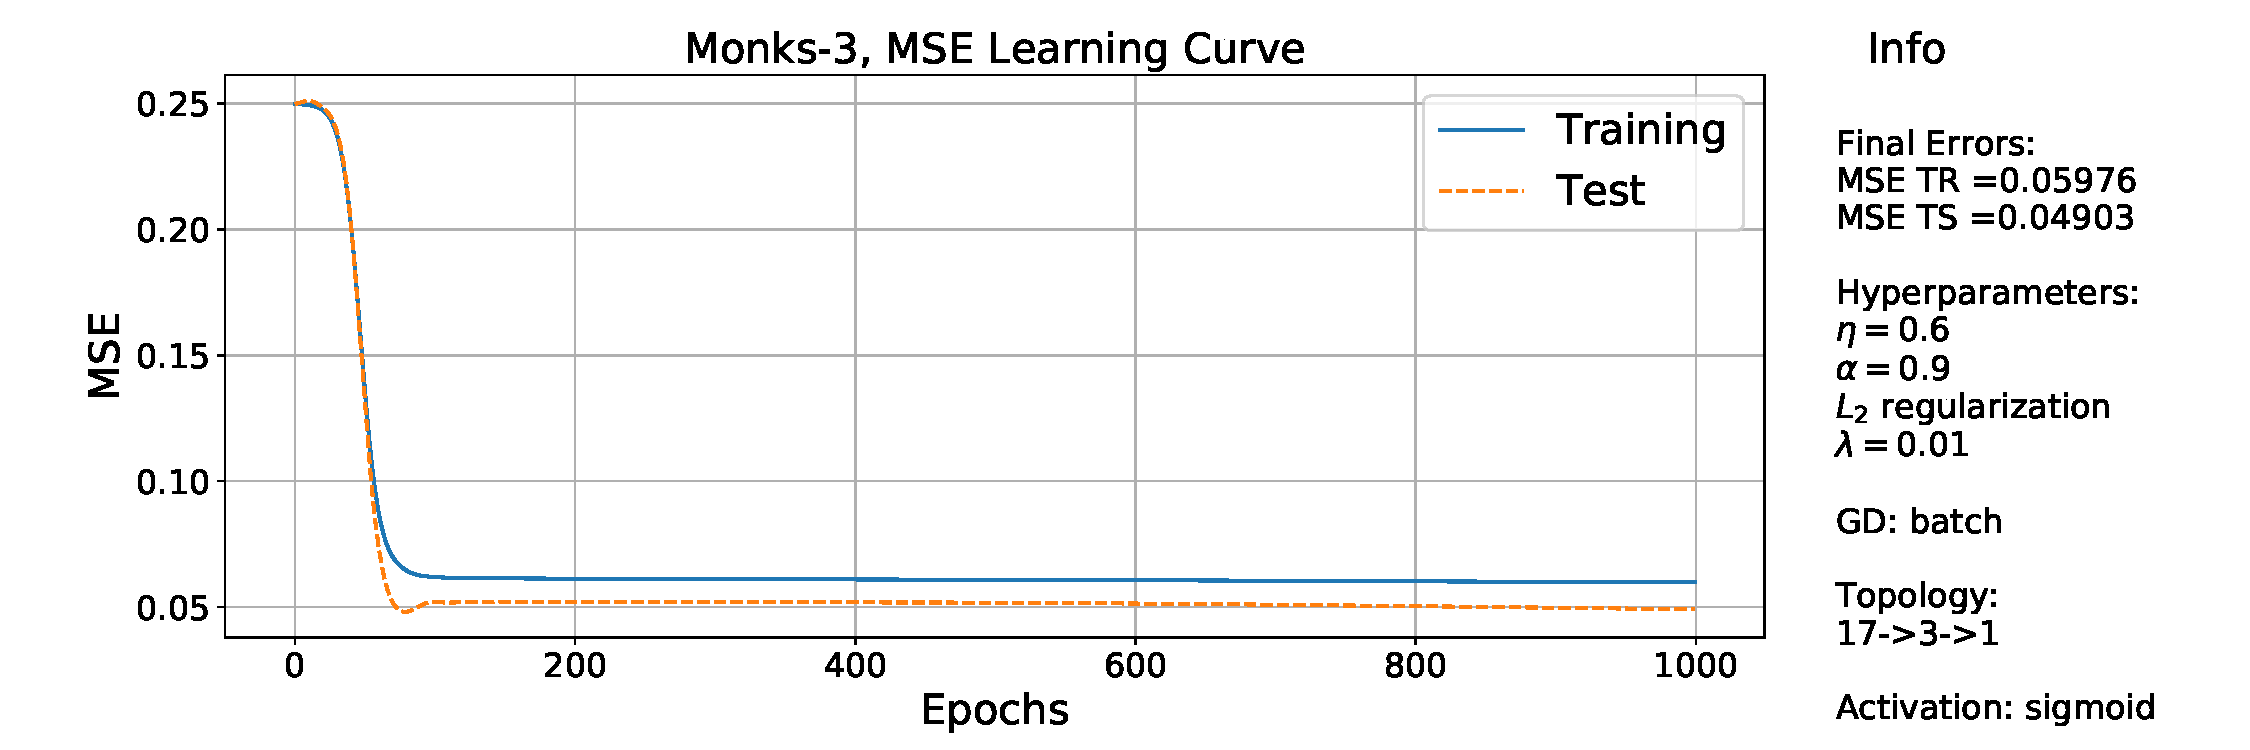
\includegraphics[width=\textwidth]{../data/monks/results/monks_3/img_final/monks_3_withreg_MSE_final_09.pdf}
  \caption{prova}
\end{figure}

\begin{figure}[htbp]
  \centering
  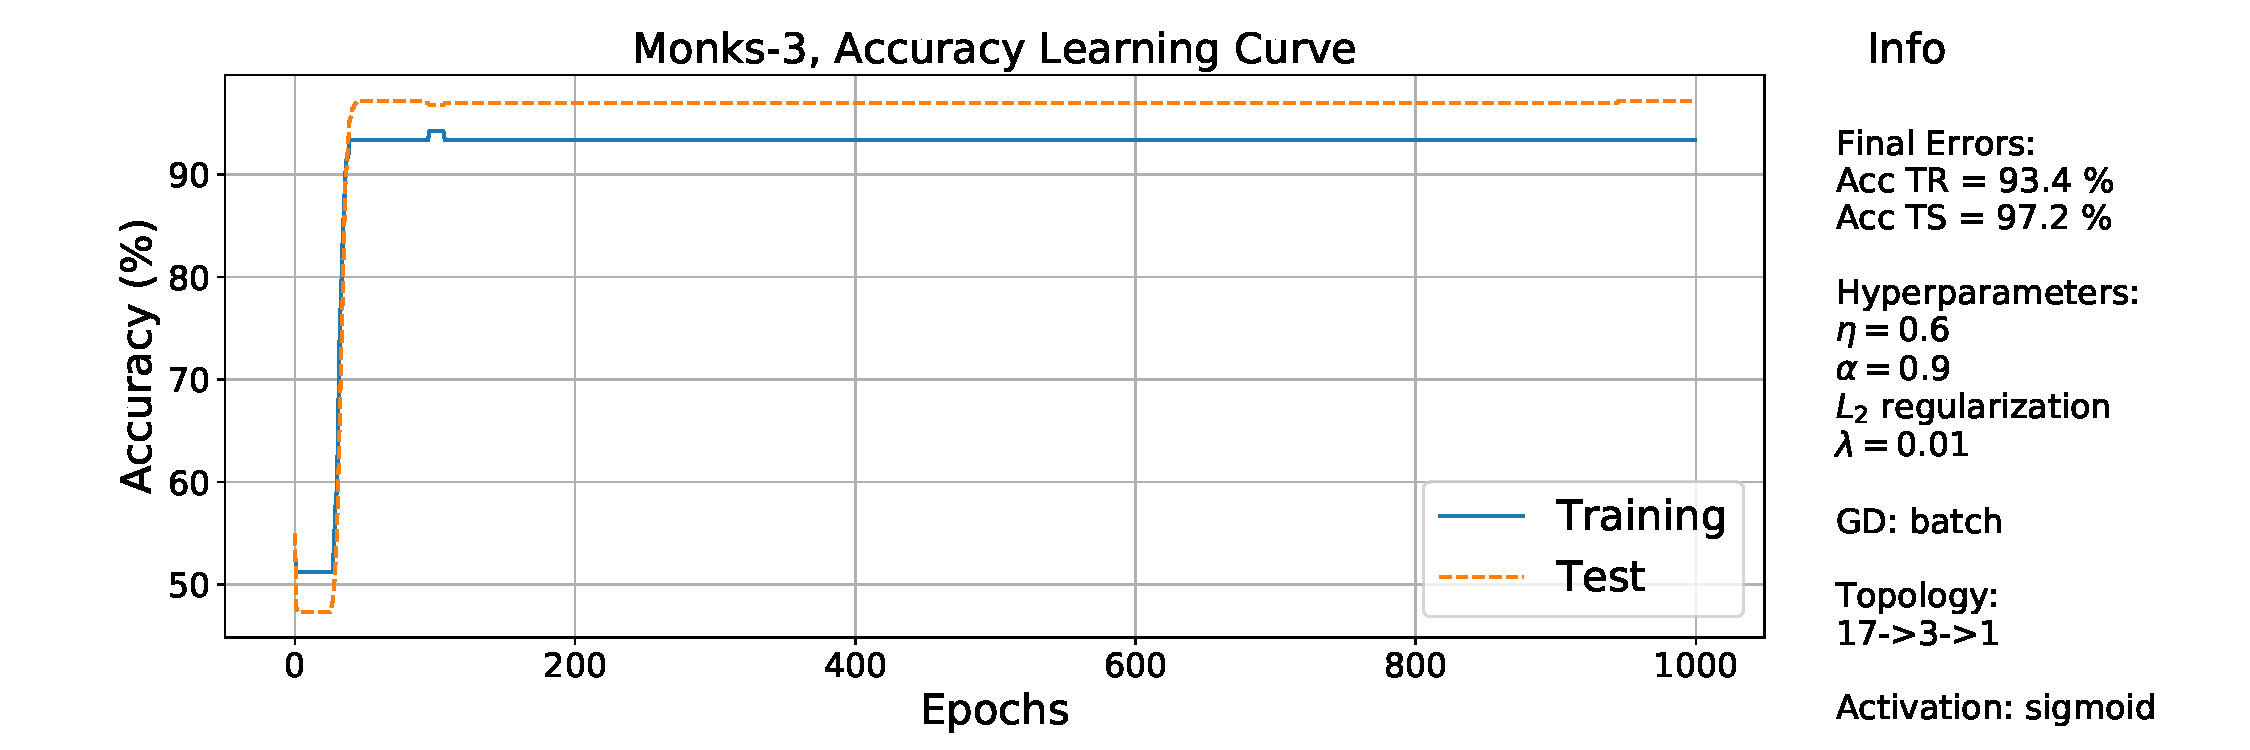
\includegraphics[width=\textwidth]{../data/monks/results/monks_3/img_final/monks_3_withreg_ACC_final_09.pdf}
  \caption{prova}
\end{figure}





% section experiments (end)

%------------------------------------------------
\clearpage

\section{Conclusions} % (fold)
\label{sec:conclusions}

% section conclusions (end)

%----------------------------------------------------------------------------------------
%   REFERENCE LIST
%----------------------------------------------------------------------------------------

\begin{thebibliography}{99} % Bibliography - this is intentionally simple in this template
    \bibitem{deep_learning}
    Ian Goodfellow, Yoshua Bengio and Aaron Courville.
    \textit{Deep Learning}, MIT Press, 2016.

    \bibitem{random_search}
    James Bergstra and Yoshua Bengio.
    \textit{Random Search for Hyper-parameter Optimization}, J. Mach. Learn. Res. 13, pp. 281-305, 2012.

    \bibitem{early_stopping}
    Prechelt L..
    \textit{Early Stopping - But When?}, Montavon G., Orr G.B., Müller KR. (eds) Neural Networks: Tricks of the Trade. Lecture Notes in Computer Science, vol 7700. Springer, Berlin, Heidelberg, 2012.

    \bibitem{initialization}
    Xavier Glorot and Yoshua Bengio.
    \textit{Understanding the difficulty of training deep feedforward neural networks},
    Proceedings of the Thirteenth International Conference on Artificial Intelligence and Statistics, pp.
    249-256, 2010.
\end{thebibliography}

%----------------------------------------------------------------------------------------

\end{document}
